\section{Zielsetzung}
In diesem Versuch wird der normale als auch der anormale Zeeman-Effekt untersucht. Dieser bezeichnet die Aufspaltung und
Polarisation von Spektrallinien in einem Magnetfeld.
\section{Theorie}
\label{sec:Theorie}
Um im Folgenden die Wechselwirkung der Drehimpulse und magnetischen Momente eines Hüllenelektrons untereinander
berechnen zu können, müssen diese zunächst näher betrachtet werden.
Bei einem Hüllenelektron kann zwischen dem Bahndrehimpuls $\vec{l}$ und dem Eigendrehimpuls $\vec{s}$ mit den Beträgen
\begin{align}
  |\vec{l}|&=\sqrt{l(l+1)}\hbar\; \text{und}\\
  |\vec{s}|&=\sqrt{s(s+1)}\hbar
\end{align}
unterschieden werden. Mit dem Bohrschen Magneton
\begin{equation}
  \mu_B=-\frac{1}{2}\cdot \frac{e_0\cdot\hbar}{m_0}
  \label{eqn:bohr}
\end{equation}
kann das magnetische Moment für den Drehimpuls als
\begin{equation}
  \vec{\mu_l}=-\mu_b\cdot\frac{\vec{l}}{\bar{h}}=-\mu_B\sqrt{l(l+1)}\vec{l_e}
  \label{eqn:magl}
\end{equation}
bestimmt werden. Dabei wird mit $\vec{l_e}$ der Einheitsvektor in $\vec{l}$-Richtung bezeichnet.
Das magnetisch Moment des Spins folgt aus dem Stern-Gerlach-Versuch und lautet
\begin{equation}
  \vec{\mu_s}\-g_S\cdot\frac{\mu_B}{\hbar}\vec{s}=-g_s \mu_B\sqrt{s(s+1)}\vec{s_e}.
  \label{eqn:mags}
\end{equation}
Dabei bezeichnet $g_s$ den Lande-Faktor, welcher hier ca. den Wert 2 besitzt. Daraus folgt die
magnetomechanische Anomalie des Elektrons, welche bezeichnet, dass $\mu_s$ etwa doppelt
so groß ist wie $\mu_l$.

Um die im allgemeinen komplexen Wechselwirkungen von Drehimpulsen und magnetischen Momenten
zu untersuchen, werden im Folgenden zwei Grenzfälle betrachtet.
\\
Zunächst wird der Fall niedriger Kernladungszahlen betrachtet.
Hier ist die Wechselwirkung zwischen den Dahndrehimpulsen dominant, somit können diese zu einem
Gesamtdrehimpuls $\vec{L}$ der Hülle addiert werden. Dabei werden nur die Drehimpulse von
nicht abgeschlossenen Schalen berücksichtigt, da abgeschlossene Schalen den Drehimpuls  Null
besitzen. Da es nur Gesamtdrehimpulse gibt, deren Quantenzahl ganzzahlig ist, ist der
Gesamtdrehimpuls eine quantisierte Größe. Zu den Quantenzahlen 0, 1, 2, 3 gehören die
S-, P-, D- und F-Terme.
Aus \ref{eqn:magl} lässt sich analog das Magnetische Moment des Gesamtdrehimpulses zu
\begin{equation}
  |\vec{\mu_{L}}|=\mu_B \sqrt{L(L+1)}
\end{equation}
bestimmen.
Äquivalent zum Gesamtdrehimpuls der Hülle gibt es einen Gesamtspin, welches sich aus der
Summe der Einzeldrehimpulse $\vec{s}$ berechnet. Die Quantenzahlen des Gesamtspin können
sowohl ganzzahlig, als auch halbzahlig sein, mit
$\frac{N}{2}$, $\frac{N}{2} -1$,..., $\frac{1}{2}$ und 0. Dabei bezeichnet $N$ die
Gesamtzahl an Elektronen in den unabgeschlossenen Schalen.
Aus Gleichung \ref{eqn:mags}ergibt sich das magnetische Moment des Gesamtspins zu
\begin{equation}
  |\vec{\mu_S}|=g_S\mu_B \sqrt{S(S+1)}.
\end{equation}

Für den Fall schwacher äußerer Magnetfelder, welcher in diesem Versuch angenommen wird, koppeln
der Gesamtdrehimpuls der Hülle $\vec{L}$ und der Gesamtspin $\vec{S}$ zum Gesamtdrehimpuls $\vec{J}$.
Der daraus entstehende Gesamtdrehimpuls $\vec{J}$ kann über die Addition
\begin{equation}
  \vec{J}=\vec{S}+\vec{L}
\end{equation}
berechnet werden. Diese Kopplung wird als LS-Kopplung bezeichnet. Aus der ganzzahligen Quantenzahl des Hüllendrehimpulses und der
ganz- oder halbzahligen Quantenzahl des Gesamtspins ergibt sich, dass die
Quantenzahl des Gesamtdrehimpulses $\vec{J}$ entweder ganz- oder halbzahlig sein kann.
Sie berechnet sich nach
\begin{equation}
  |\vec{J}|=\sqrt{J(J+1)}\hbar.
\end{equation}
\\
Für den Fall hoher Kernladungszahlen überwiegt die Wechselwirkung zwischen
Bahndrehimpuls und Spin, welche als jj-Kopplung bezeichnet wird.
Die Wechselwirkung der Größen $\vec{l_i}$ bzw. $\vec{s_i}$ untereinander ist deutlich
schwächer, wodurch kein Gesamtspin $\vec{S}$ und kein Gesamtdrehimpuls $\vec{L}$ existiert.
Für diesen Fall setzen sich $\vec{l_i}$ und $\vec{s_i}$ zu den Gesamtdrehimpulsen
\begin{equation}
  \vec{j_i}=\vec{l_i} +\vec{s_i}
\end{equation}
der Einzelelektronen zusammen. Die Summer dieser Einzeldrehimpulse bildet
den Gesamtdrehimpuls $\vec{J}$.

\subsection{Aufspaltung der Energieniveaus im homogenen Magnetfeld}
Das zum Gesamtdrehimpuls $\vec{J}$ gehörende magnetisch Moment setzt sich aus den
magnetischen Momenten $\vec{\mu_s}$ und $\vec{\mu_s}$ zusammen:
\begin{equation}
  \vec{\mu}=\vec{\mu_s}+ \vec{\mu_L}
  \label{eqn:magges}
\end{equation}
Dabei lässt sich der Betrag über die Formel
\begin{equation}
  |\vec{\mu_J}|=\mu_B g_J\sqrt{J(J+1)}
  \label{eqn:muJ}
\end{equation}
mit dem Lande-Faktor
\begin{equation}
  g_J=\frac{3J(J+1)+S(S+1)-L(L+1)}{2J(J+1)}
  \label{eqn:gJ}
\end{equation}
bestimmen.

Des Weiteren treten bei Eingeschaltetem äußeren Magnetfeld aufgrund der
Richtungsquantelung nur Winkel auf, die ein ganzzahliges Vielfaches von
$g_J \mu_B$ sind, also
\begin{equation}
  \mu_{J_z}=-mg_J \mu_B
  \label{eqn:richtung}
\end{equation}
erfüllen. Dabei ist $m$ die ganzzahlige Orientierungsquantenzahl, welche
Werte zwischen -J,-J+1,...,0,1,...,J annehmen kann. Somit hat das
atomare magnetische Moment $2J+1$ Einstellmöglichkeiten gegenüber dem
äußeren Feld. Über die Formel
\begin{equation}
  E_{mag}=-\vec{\mu_J}\cdot\vec{B}\:\:\:\text{bzw.}\:\:\:E_{mag}=mg_J \mu_B
  \label{eqn:emag}
\end{equation}
lässt sich nun die Energie berechnen, die das magnetische Moment
im Magnetfeld erhält. Daraus folgt, dass das Energieniveau $E_=0$
unter Einfluss eines äußeren Magnetfeldes in $2J+1$ äquidistante
Niveaus aufspaltet.
Diese Aufspaltung tritt sowohl im Grundzustand, als auch bei
angeregten Zuständen auf. Daher treten bei Eingeschaltetem
äußerem Magnetfeld zusätzliche Übergänge zwischen den neu entstandenen
Niveaus auf. Ob eine neue Spektrallinie entsteht ist davon abhängig, welche
Übergänge möglich sind. Dies wird durch die
Auswahlregeln festgelegt.

Zur Bestimmung der Auswahlregeln wird zunächst die zeitabhängige
Schrödingergleichung
\begin{equation}
  -\frac{\hbar^2}{2m}\Delta\psi(\vec{r},t)+U\psi(\vec{r},t)+\frac{\hbar}{i}\frac{\partial\psi(\vec{r}),t}{\partial t}=0
\end{equation}
gelöst. Die Lösung setzt sich als Linearkombination zweier Lösungen für
die an dem Übergang beteiligten Energieniveaus zusammen:
\begin{equation}
  \psi_{ges}(\vec{r},t)=C_{\alpha}\psi_{\alpha}(\vec{r})\exp(-\frac{i}{\hbar}E_{\beta}t)+
  C_{\beta}\psi_{\beta}(\vec{r})\exp(-\frac{i}{\hbar}E_{\beta}t).
\end{equation}
Dabei bezeichnen $E_{\alpha}$ und $E_{\beta}$ die beteiligten Energieniveaus, zwischen denen
der Übergang stattfindet. Durch eitere Rechnungen lässt sich zeigen, dass Übergänge
nur für
\begin{equation}
  \Delta m= 0,-1 \;\text{und}\;+1
\end{equation}
stattfinden. Für den Fall $\Delta m=0$ ergibt sich, dass die emittierte
Strahlung  parallel zu $\vec{B}$ linear-polarisiert ist. Für $\Delta m= -1, +1$
ist die emittierte Strahlung um die z-Achse zirkular polarisiert.

\subsection{Normaler und Anormaler Zeeman-Effekt}
Die bisherigen Ergebnisse basieren auf der zeitabhängigen Schrödingergleichung,
welche den Spin vernachlässigt. Daher sind die bisherigen Ergebnisse nur für den
Fall $S=0$ gültig, welcher als normaler Zeeman-Effekt bezeichnet wird.
Für diesen Fall ergibt sich aus Gleichung \ref{gJ}, dass für $S=0$ immer
$g_j=1$ gilt. Damit ist nach Gleichung \ref{fig:emag} die Verschiebung der
Energieniveaus unabhängig von den Quantenzahlen und es gilt:
\begin{equation}
  \Delta E =m \mu_B B
\end{equation}

\begin{figure}
  \centering
  \includegraphics[width=11cm]{Übergang.png}
  \caption{Termschema für die Zeemann-Übergänge $\Delta m=\pm1, 0$ \cite{demtröder}. }
  \label{fig:Übergang}
\end{figure}


In Abbildung \ref{fig:Übergang} ist ein Termschema für die Zeeman-Übergänge
$\Delta m=\pm1, 0$ dargestellt. Es treten drei Liniengruppen auf die $\Delta m=1$,
$\Delta m=-1$ oder $\Delta m=0$ zugeordnet werden können. Die Enrgiedifferenzen
innerhalb einer dieser Gruppen mit konstantem $\Delta m $ sind konstant, weshalb
immer 3 Übergänge sichtbar sind. Dies wird auch als Zeeman-Triplett bezeichnet.
Da die emittierten Linien eine Polarisation aufweisen können sie nicht
aus jeder Beobachtungsrichtung beobachtet werden. Diese Tatsache wird durch Abbildung
\ref{fig:polar} verdeutlicht.

\begin{figure}
  \centering
  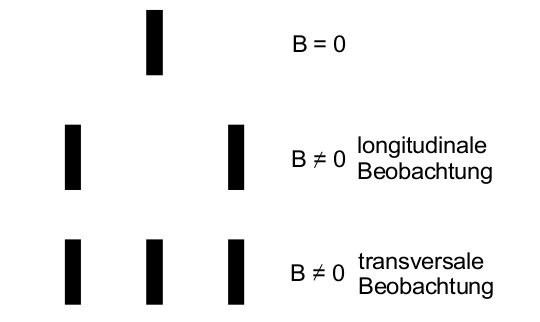
\includegraphics[height=6cm]{Punkt.png}
  \caption{Spektrallinien beim normalen Zeemann-Effekt in abhängigkeit
  der Beobachtungsrichtung.\cite{anleitung}}
  \label{fig:polar}
\end{figure}

Die durch $\Delta m=0$ erzeugte Linie ist linear in Feldrichtung polarisiert und
wird auch als $\pi$-Komponente bezeichnet. Sie ist bei einer Beobachtungsrichtung
transversal zu Feldrichtung beobachtbar. Als $\sigma$-Komponenten
werden die Linien mit $\Delta m=\pm1$ bezeichnet, welche zirkular um die
Feldachste polarisiert sind. Bei transversaler Beobachtungsrichtung erscheinen
sie linear polarisiert.
\\

Der Unterschied des anormalen Zeeman-Effekts zum normalen Zeeman-Effekt ist, dass
der Spin mit berücksichtigt wird. Es lässt sich mit der spinabhängigen
Schödinger-Gleichung zeigen, dass die Auswahlregeln
$\Delta m=\pm1,0$ auch für den Fall $S\neq0$ gelten. Damit wird die Aufspaltung
vielfältiger, da nicht mehr $g=1$ gilt, sondern von $L$, $S$ und $J$ abhängt.
